\documentclass[a4paper,11pt]{article}
\usepackage[utf8]{inputenc}
\usepackage[T1]{fontenc}
\usepackage[french]{babel}
\usepackage{textcomp}
\usepackage{amsmath,amssymb}
\usepackage[coverpage,fancysections]{polytechnique}
%\usepackage[fancysections]{polytechnique}
\usepackage{graphicx}


\def \P{\mathbb{P}}
\def \E{\mathcal{E}}
\def \esp{\mathbb{E}}

\title{Retour vers le futur}
\author{Qi \textsc{Sun} et Victor \textsc{Quach}}
\date{}

\begin{document}
\maketitle


\subsection*{T1}

\begin{itemize}
\item[\textbullet]
Soit $k \in \E^{bin}=\{0, \dots, M\}$. 

Compte-tenu, de la définition de $F^{bin}$, on a \underline{pour $k<M$} :


\begin{center}
\fbox{\begin{minipage}{0.5\textwidth}
\[P^{bin}(k,k+1) = p\frac{M-k}{M}\]
\end{minipage}}
\end{center}

Notons que le membre de droite est nul pour $k=M$.\\


De même, \underline{pour $k>0$} : 
\begin{center}
\fbox{\begin{minipage}{0.5\textwidth}
\[P^{bin}(k,k-1) = (1-p)\frac{k}{M}\]
\end{minipage}}
\end{center}
Le membre de droite est nul pour $k=0$.\\


Il vient donc, \underline{pour $k \in \E^{bin}$},
\begin{center}
\fbox{\begin{minipage}{0.5\textwidth}
\[P^{bin}(k,k) = 1 - p +\frac{2kp}{M}+\frac{k}{M}\]
\end{minipage}}
\end{center}

\vspace{5mm}
Enfin, \underline{pour $x,y \in \E^{bin}$, si $|x-y|>1$},
\begin{center}
\fbox{\begin{minipage}{0.5\textwidth}
\[P^{bin}(x,y) = 0\]
\end{minipage}}
\end{center}
\vspace{5mm}



\item[\textbullet]
Soit $x,y \in \E^{bin}$.

En utilisant que $\pi^{bin}(x)  = \binom{M}{x}p^x(1-p)^{M-x}$, il vient dans les différents cas :

	\begin{itemize}
		\item 	Si $(x,y) = (k,k+1)$
			\begin{equation*}	
			\begin{split}
			\pi^{bin}(k)P(k,k+1) &= \binom{M}{k}p^k(1-p)^{M-k}p\frac{M-k}{M} \\
			&= \frac{M-k}{M}\binom{M}{M-k}p^{k+1}(1-p)^{M-k-1}(1-p)\\
			&= \binom{M-1}{M-k-1}p^{k+1}(1-p)^{M-k-1}(1-p)\\
			&= \binom{M-1}{k}p^{k+1}(1-p)^{M-k-1}(1-p)\\
			&= \frac{k+1}{M}\binom{M}{k+1}p^{k+1}(1-p)^{M-k-1}(1-p)\\
			&= \pi^{bin}(k+1)P(k+1,k) 
			\end{split}
			\end{equation*}
		\item   Si $(x,y) = (k,k)$, L'équation est trivialement vérifiée
		\item   Sinon, les deux memmbres sont nuls.
	\end{itemize}
		Finalement, pour tout $x,y \in \E^{bin}$, 
\begin{center}
\fbox{\begin{minipage}{0.5\textwidth}
\[\pi^{bin}(x)P(x,y) = \pi^{bin}(y)P(y,x) \]
\end{minipage}}
\end{center}

\item[\textbullet]
Soit $X$ une variable aléatoire de loi $\pi^{bin}$. Alors, pour $x\in \E$,
\begin{equation*}
\begin{split}
 \P(F^{bin}(X)=x) &= \sum_{y\in\E}{\pi^{bin}(y)P^{bin}(y,x)}
		  = \sum_{y\in\E}{\pi^{bin}(x)P^{bin}(x,y)}\\
		  &= \pi^{bin}(x)P\sum_{y\in\E}{^{bin}(x,y)}
		  = \pi^{bin}(x)\\
		  &= \P(X=x) 
\end{split}
\end{equation*}
\begin{center}
\fbox{\begin{minipage}{0.5\textwidth}
De cela, on déduit que $\pi^{bin}$ est invariante pour $F^{bin}$.
\end{minipage}}
\end{center}

\end{itemize}


\subsection*{S1}
En faisant varier les paramètres de la simulation ($p$, $M$, $n$), on obtient toujours le résultat représenté à la \textsc{figure} \ref{S1} : $X_n = F^{bin}_{n,0}$ suit la loi binomiale $\text{Bin}(M,p)$.
\begin{figure}[h]
\center
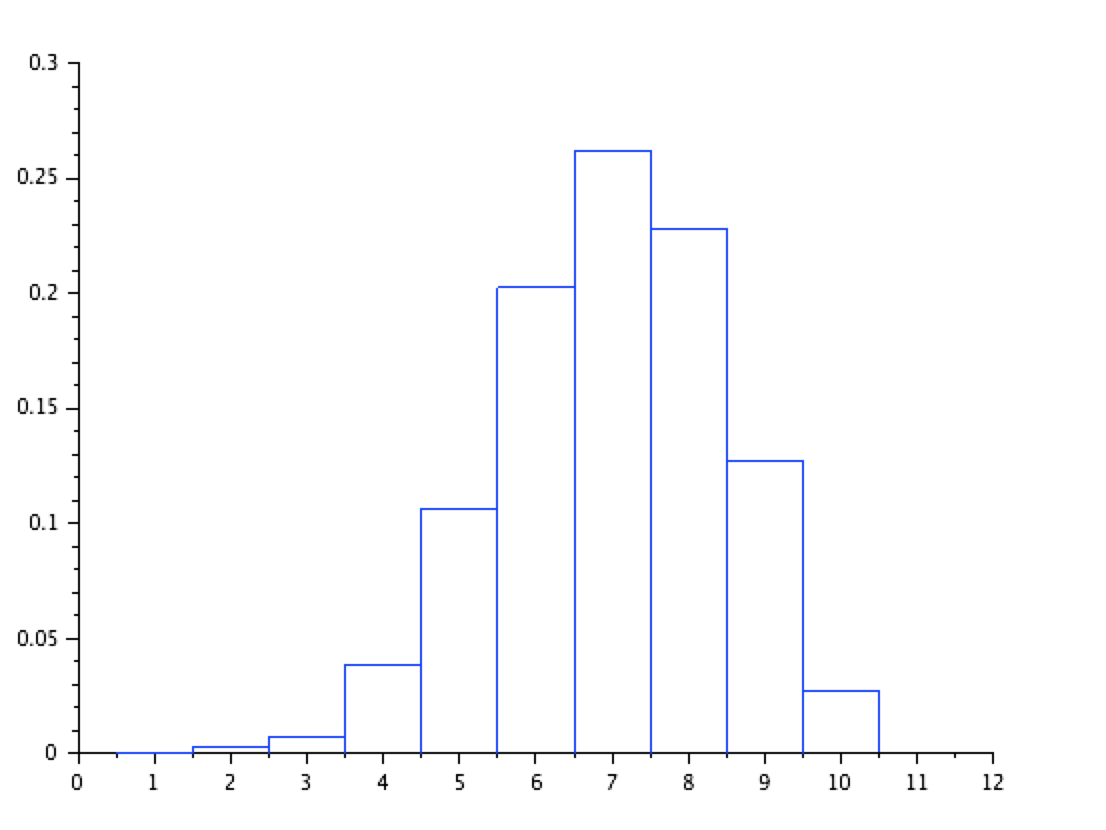
\includegraphics[width=11cm]{S1}
\caption{Histogramme de $X_{15}$ pour $p=0.7$, $M=10$, 5000 lancers}
\label{S1}

\end{figure}

\section{Coalescence et loi invariante}
\subsection*{S2}
On représente $n$ sur l'axe des abscisses et $F_n^{bin}(x)$ sur l'axe des ordonnés pour trois trajectoires rouge, bleue et rose. Sur la \textsc{figure} \ref{S2}, rose et bleu coalescent à la 28\ieme{} itération, puis avec rouge à la 36\ieme{}.
\begin{figure}[h]
\center
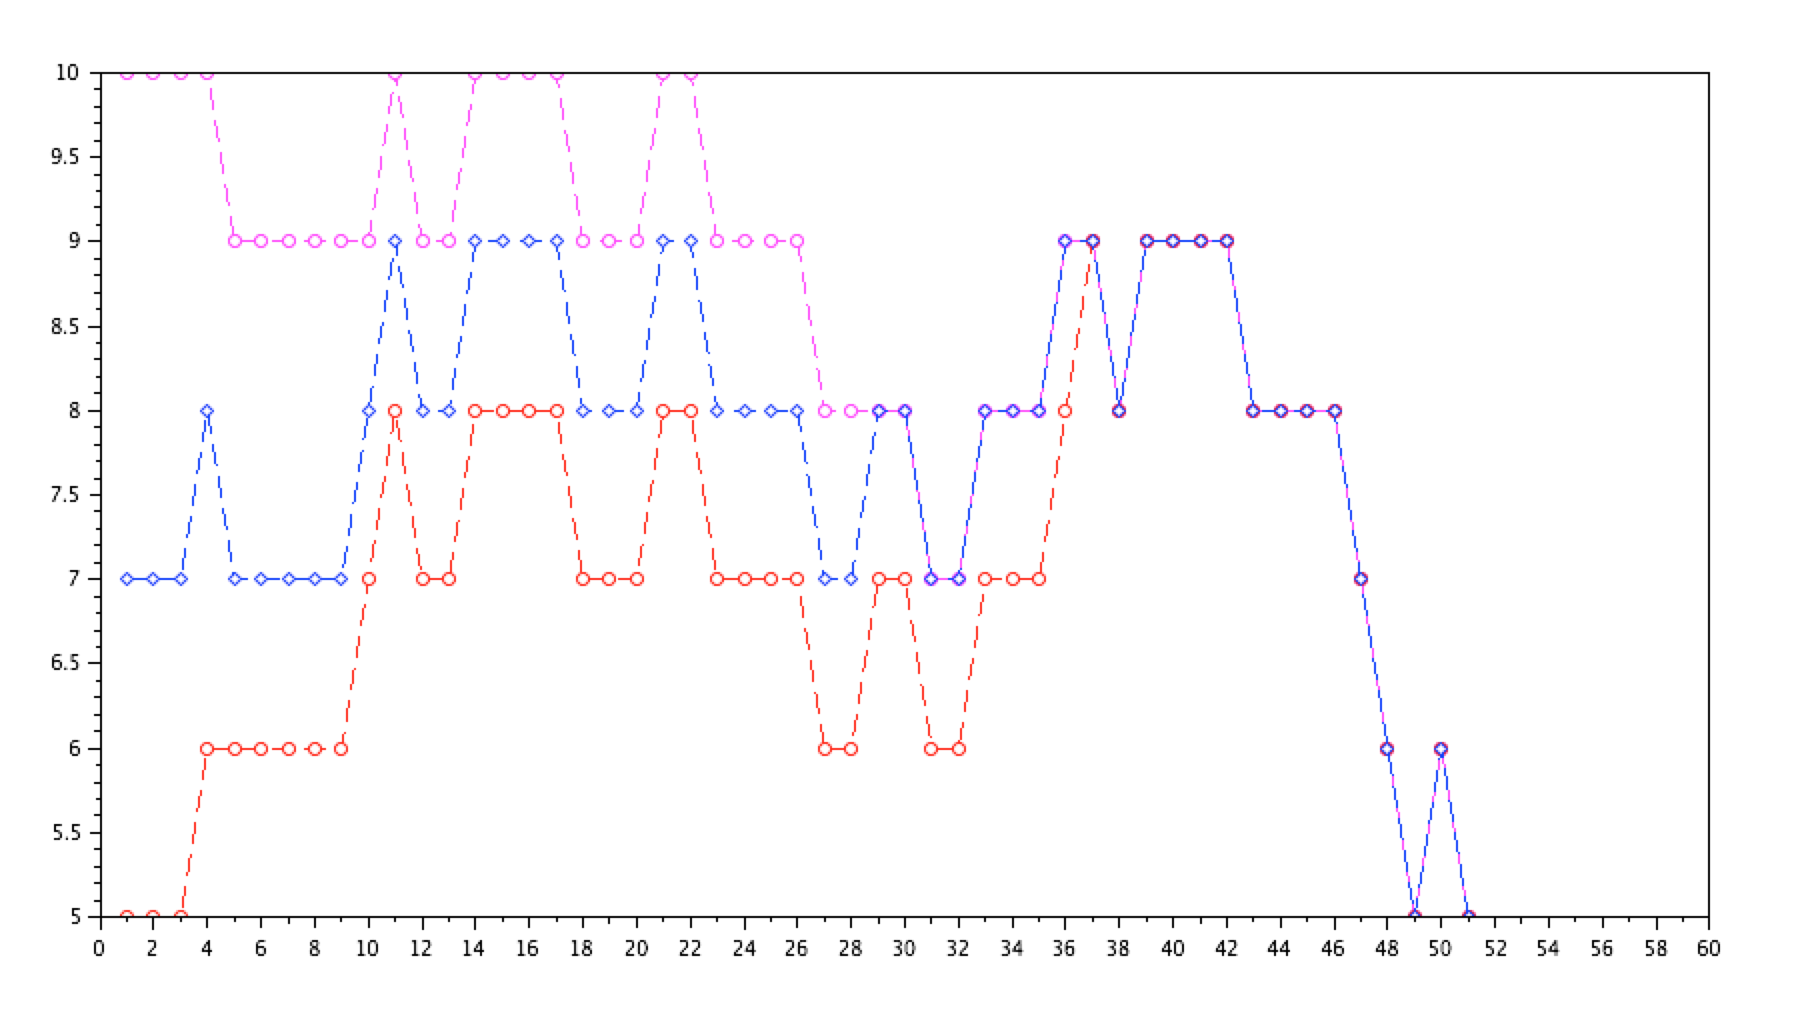
\includegraphics[width=15cm]{S2}
\caption{Coalescence de trois trajectoires du système dynamique $F^{bin}$}
\label{S2}

\end{figure}


\subsection*{T2}
\begin{itemize}

\item[\textbullet]
Il s'agit de calculer :
\begin{equation*}
\begin{split}
\mathbb{P}(A_1)&=\mathbb{P}(\{F_{0,{n_0}k}(X)=F_{0,{n_0}k}(Y)\})\\
&=\sum_{x,y} \mathbb{P}(F_{0,{n_0}k}(x)=F_{0,{n_0}k}(y))\mathbb{P}(X=x,Y=y)
\end{split}
\end{equation*}
Or, on a supposé que :
\[\inf_{x,y}\mathbb{P}(F_{0,{n_0}k}(x)=F_{0,{n_0}k}(y))\geq\varepsilon>0\]
D'où :
\[ \mathbb{P}(A_1)\geq\sum_{x,y} \varepsilon\mathbb{P}(X=x,Y=y)\geq\varepsilon\sum_{x,y}\mathbb{P}(X=x,Y=y)\geq\varepsilon\]
Ainsi,
\begin{center}
\fbox{\begin{minipage}{0.5\textwidth}
\[ \mathbb{P}(A_1)\geq\varepsilon\]
\end{minipage}}
\end{center}

\item[\textbullet]
Montrons par récurrence sur $l$ que:
\begin{center}
\fbox{\begin{minipage}{0.5\textwidth}
\[ \mathbb{P}(S>l)=\mathbb{P}({A_1}^c,{A_2}^c,...,{A_l}^c)\le(1-\varepsilon)^l. \]
\end{minipage}}
\end{center}
Le résultat au rang $1$ se déduit du point précédent.
Soit $l\geq1$, supposons le résultat au rang $l$. Alors
\begin{equation*}
\begin{split}
\mathbb{P}(S>l+1)&=\mathbb{P}({A_1}^c,{A_2}^c,...,{A_l}^c,{A_{l+1}}^c)\\
&=\sum_{x,y} \mathbb{P}(F_{0,n_0}(x)\neq F_{0,n_0}(y),...,F_{0,{n_0}(l+1)}(x)\neq F_{0,{n_0}(l+1)}(y))\mathbb{P}(X=x,Y=y)\\
%\begin{multline*}
&=\sum_{x,y} \mathbb{P}(F_{n_0l,n_0(l+1)}(F_{0,{n_0}l}(x))\neq F_{n_0l,n_0(l+1)}(F_{0,{n_0}l}(y))) \\
&\hspace{1cm}\times\mathbb{P}(F_{0,n_0}(x)\neq F_{0,n_0}(y),...,F_{0,{n_0}l}(x)\neq F_{0,{n_0}l}(y))\mathbb{P}(X=x,Y=y)\\
%\end{multline*}
&\leq (1-\varepsilon)\mathbb{P}(S>l)\\
&\leq (1-\varepsilon)^{(l+1)}
\end{split}
\end{equation*}
D'où le résultat par récurrence.
On en déduit:
\[\mathbb{E}[S]=\sum_{l\geq0}\mathbb{P}(S>l)\leq\sum_{l\geq0}(1-\varepsilon)^l\]
Finalement :

\begin{center}
\fbox{\begin{minipage}{0.5\textwidth}
\[\mathbb{E}[S]\leq\frac{1}{\varepsilon}\]
\end{minipage}}
\end{center}

\item[\textbullet]
D'une part, $(\mathbb{P}(F_{0,n}(X)=F_{0,n}(Y)))_n\in \mathbb{N}$ est une suite croissante sur $n$.\\
D'autre part, pour tout $n\geq 1$, $\mathbb{P}(F_{0,nn_0}(X)=F_{0,nn_0}(Y))\geq\mathbb{P}(S\leq n)$.\\
Ainsi,
\[1-(1-\varepsilon)^n\leq\mathbb{P}(F_{0,nn_0}(X)=F_{0,nn_0}(Y))\leq1\]
D'après le théorème d'encadrement et la monotonie de la suite, il vient :

\begin{center}
\fbox{\begin{minipage}{0.5\textwidth}
\[\lim\limits_{n \rightarrow +\infty} \mathbb{P}(F_{0,n}(X)=F_{0,n}(Y)) = 1\]
\end{minipage}}
\end{center}

\end{itemize}

\subsection*{T3}
Supposons que $\pi$ et $\nu$ sont deux probabilités invariantes. 
Alors pour tout $n\geq0$, $F_{0,n}(X)$ suit la même loi que $X$, ainsi que $Y$.
Soit $\varphi$ une fonction continue bornée,
\[\mathbb{E}(\varphi(X-Y))=\mathbb{E}(\varphi(F_{0,n}(X)-F_{0,n}(Y)))\]
$\varphi(F_{0,n}(X)-F_{0,n}(Y))$ converge en probabilité(d'après la question $T2$), donc en loi vers $0$.
D'où:
\[\mathbb{E}(\varphi(X-Y))=\lim \limits_{n \rightarrow +\infty}\mathbb{E}(\varphi(F_{0,n}(X)-F_{0,n}(Y)))=0\]
Donc $X$ et $Y$ suivent la même loi, i.e. $\pi = \nu$.
\underline{Ainsi, il existe au plus une probabilité invariante}.

\subsection*{T4}
Soient $x,y \in \E$.
On peut montrer par récurrence (de même que dans la question \textbf{T2.}) que:

\[\forall l\geq 0, \quad \P(T_+^{x,y}>n_0l)=\P(F_{0,n_0l}(x)\ne F_{0,n_0l}(y))\leq (1-\varepsilon)^l\]
Par ailleurs, $(P(T_+^{x,y}>n)_{n \in \mathbb{N}}$ est une suite décroissante, d'où :
\[\forall l, \forall n, \quad n_0l\leq n \leq n_0(l+1) \Rightarrow \P(T_+^{x,y}>n) \leq (1-\varepsilon)^l \]
Ainsi: 
\[ \esp[T_+^{x,y}]  = \sum_{n\geq 0} \P(T_+^{x,y}>n) \le  \sum_{n\geq 0} (1-\varepsilon)^{\left\lfloor\frac{n}{n_0}\right\rfloor} = \frac{n_0}{\varepsilon} \] 
Les variables aléatoires $T_+^{x,y}$ étant positives, on a :

\[ T_+ = \max_{x,y}  T_+^{x,y} \le \sum_{x,y} T_+^{x,y} \] 
D'où l'on déduit que:
\begin{equation*}
\begin{split}
\mathbb{E}[T_+] & \le \esp[\sum_{x,y} T_+^{x,y}] \\
		& \le \sum_{x,y} \esp[T_+^{x,y}]  \\
		& \le \binom{\# \E}{2} \frac{n_0}{\varepsilon} 
\end{split}
\end{equation*}
\underline{Ainsi, $\E[T_+]$ est fini et borné par $\binom{\# \E}{2} \frac{n_0}{\epsilon}$.}

\subsection*{T5}
\begin{itemize}

\item[\textbullet]
Montrons par récurrence que $F_{0,n}(x) \sim F_{-n,0}(x)$ pour tout $x \in \E$ et $n \in \mathbb{N}$:

Soit $x \in \E$, $n=0$, on a directement:
\[F_{0,0}(x)=F_{-0,0}(x)\]
Soit $n \geq 0$, supposons le résultat au rang $n$, alors soient $x,y \in \E$,
\begin{equation*}
\begin{split}
\P(F_{-(n+1),0}(x)=y)&=\P(F_0\circ F_{-(n+1),-1}(x)=y)\\
&=\sum_{z \in \E} \P(F_0(z)=y)\P(F_{-(n+1),-1}(x)=z)\\
&=\sum_{z \in \E} \P(F_{n+1}(z)=y)\P(F_{0,n}(x)=z) \quad\quad\text{(d'après H.R.)}\\
&=\P(F_{n+1}\circ F_{0,n}(x)=y)\\
&=\P(F_{0,n+1}(x)=y)
\end{split}
\end{equation*}
Ainsi, $F_{-(n+1),0}(x) \sim F_{0,n+1}(x)$.
D'où le résultat par récurrence sur $n$.\\
\\
\item[\textbullet]
Soit $n \in \mathbb{N}$,
\begin{equation*}
\begin{split}
\P(T_{+}\leq n)&=\sum_{z \in \E} \prod_{x \in \E} \P(F_{n,0}(x)=z)\\
&=\sum_{z \in \E} \prod_{x \in \E} \P(F_{0,-n}(x)=z)\\
&=\P(T_{-}\leq n)
\end{split}
\end{equation*}
$T_+$ et $T_-$ ont donc la même fonction de répartition.
\underline{Ainsi, $T_+ \sim T_-$.}\\
\\
\item[\textbullet]
Soient $x \in \E$ et $n \geq T_-$,
\[\underline{F_{-n,0}(x)}=F_{-T_-,0}(F_{-n,-T_-}(x))=\underline{F_{-T_-,0}(x)}\]\\
Soit $x \in \E$:
\begin{equation*}
\begin{split}
\P(F(X^*) = x) &= \P(F\circ F_{-T,0}(x_0) = x) \\
	      &= \sum_{y \in \E}\P(F_{-T_-,0}(x_0)=y)\P(F(y)=x)\\
	      &= \sum_{y \in \E}\P(F_{0,T_-}(x_0)=y)\P(F_{T_-+1}(y)=x)\\
	      &= \P(F_{0,T_-+1}(x_0)=x)\\
	      &= \P(F_{-(T_-+1),0}(x_0)=x)\\
	      &= \P(F_{-T_-,0}(x_0)=x)\\
	      &= \P(X^*=x)
\end{split}
\end{equation*}
La loi de $X^*$ est donc invariante par $F$. D'après l'unicité de probabilité invariante montrée dans la question T3, on a:

\begin{center}
\fbox{\begin{minipage}{0.5\textwidth}
\[X^* \sim \pi\] 
\end{minipage}}
\end{center}

\end{itemize}

\subsection*{S3}
Contrairement à ce que l'on espérait la simulation aboutit à un histogramme qui ressemble méchamment à celui d'une loi binomiale $\text{Bin}(M,p)$.
\begin{figure}[h]
\center
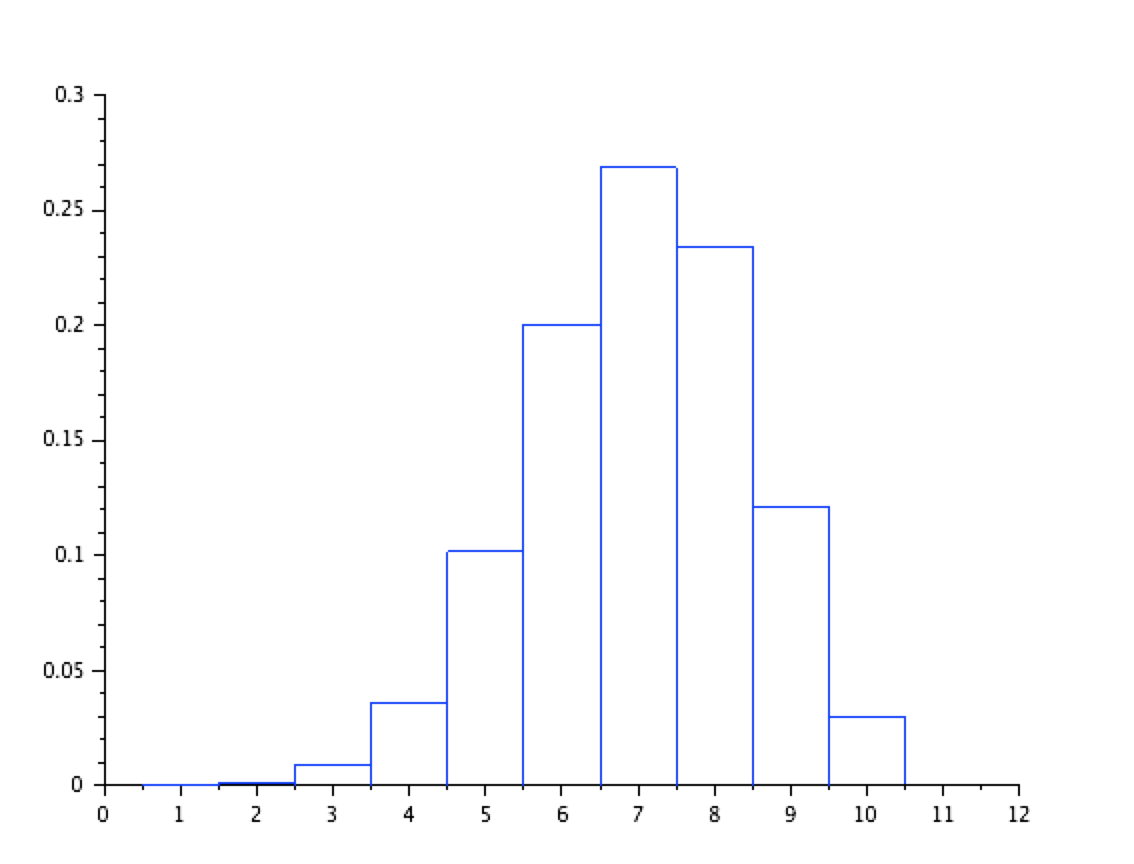
\includegraphics[width=11cm]{S3}
\caption{Histogramme de $X^{**}$ pour $p=0.7$, $M=10$, 5000 lancers}
\label{S3}

\end{figure}


\section{Couplage monotone}

\subsection*{T6}

Il s'agit de montrer que $F^{bin}$ est croissante sur $(\E^{bin},\le)$.

Soit $x,y \in \E^{bin}$, avec $x\le y$. Si $x=y$, le résultat est assuré. Supposons $x<y$. On distingue les cas selon les valeurs de $K$ et $U$. 
\vspace{0.5cm}

\begin{itemize}
\item[\textbullet] Si $U>p$
	\begin{itemize}
	\item Si $x<y<K$, $F^{bin}(x) = x < y = F^{bin}(y)$
	\item Si $x<K\le y$, $F^{bin}(x) = x \le y-1 = F^{bin}(y)$
	\item Si $K\le x < y$, $F^{bin}(x) = x - 1 < y - 1 = F^{bin}(y)$
	\end{itemize}
\item[\textbullet] Sinon, $U\le p$.
	\begin{itemize}
	\item Si $x<y<K$, $F^{bin}(x) = x + 1 < y + 1= F^{bin}(y)$
	\item Si $x<K\le y$, $F^{bin}(x) = x +1 \le y = F^{bin}(y)$
	\item Si $K\le x < y$, $F^{bin}(x) = x < y = F^{bin}(y)$
	\end{itemize}
\end{itemize}

\begin{center}
 \underline{Finalement, $F^{bin}$ est croissante sur  $(\E^{bin},\le)$.}
\end{center}

\subsection*{T7}
Supposons que $F$ est croissante, alors $\forall n \in \mathbb{N}$, $F_{-n,0}$ est croissante. D'où :


 \[\forall x,y \in \E, F_{-n,0}(x)=F_{-n,0}(y)\quad \iff \quad F_{-n,0}(\hat{0})=F_{-n,0}(\hat{1})\]

On en déduit:
\begin{center}
\fbox{\begin{minipage}{0.5\textwidth}
\[T_-=\inf\{n\geq 0: F_{-n,0}(\hat{0})=F_{-n,0}(\hat{1})\}\] 
\end{minipage}}
\end{center}

\subsection*{T8}
Comme on a montré que $T_+ \sim T_-$ dans la question $5$, estimer $\mathbb{E}[T_-]$ revient à trouver une estimation de $\mathbb{E}[T_+]$, avec $T_+=\inf\{n\geq 0: F_{0,n}(\hat{0})=F_{0,n}(\hat{1})\}$.\\
Ainsi, d'après la question 4, on a:
\[\esp[T_+]=\esp[T_+^{\hat{0},\hat{1}}]\leq \frac{n_0}{\varepsilon}\] 
D'où:
\begin{center}
\fbox{\begin{minipage}{0.5\textwidth}
\[\esp[T_-]\leq \frac{n_0}{\varepsilon}\] 
\end{minipage}}
\end{center}

\subsection*{T9}
L'algorithme procède au calcul d'une instance de $X^*$, dont la loi est $\pi$. 

Il s'agit d'une part d'évaluer $T_-$, puis de retourner $F_{-T_-,0}(x_0$, pour un $x_0$ quelconque. Ici, on se contente de minorer $T_-$ par $kN_0$ et on choisit $x_0 = \hat{0}$, ce qui est justifié car $kN_0 \ge T_- \Rightarrow F_{-kN_0,0}(x_0) = F_{-T_-,0}(x_0)$ et cette valeur est indépendante du $x_0$ choisi.

Il est important de réutiliser les instances de $F$ générées dans les itérations précédentes, sinon on se retrouve à sélectionner une suite d'instances de $F$ avec un $T_-$ moins élevé qui, d'autre part, n'assure plus que le résultat renvoyé suive la loi $\pi$.

On choisit de doubler $N$ à chaque itération plutôt que de l'incrémenter de 1 simplement pour diminuer le temps de calcul : dans l'algorithme proposé, on choisit de ne calculer qu'une trajectoire pour $N-1$ trajectoires que l'on ne calcule pas. Cela ne permet pas de trouver explicitement $T$ mais suffit pour renvoyer une instance de $X^*$.

\subsection*{S4}
En faisant varier les paramètres $M$ et $p$, on constate que $X^{*}$ suit la loi binomiale $\text{Bin}(M,p)$, comme on le voit sur la \textsc{figure} \ref{S4}. 
\begin{figure}[h]
\center
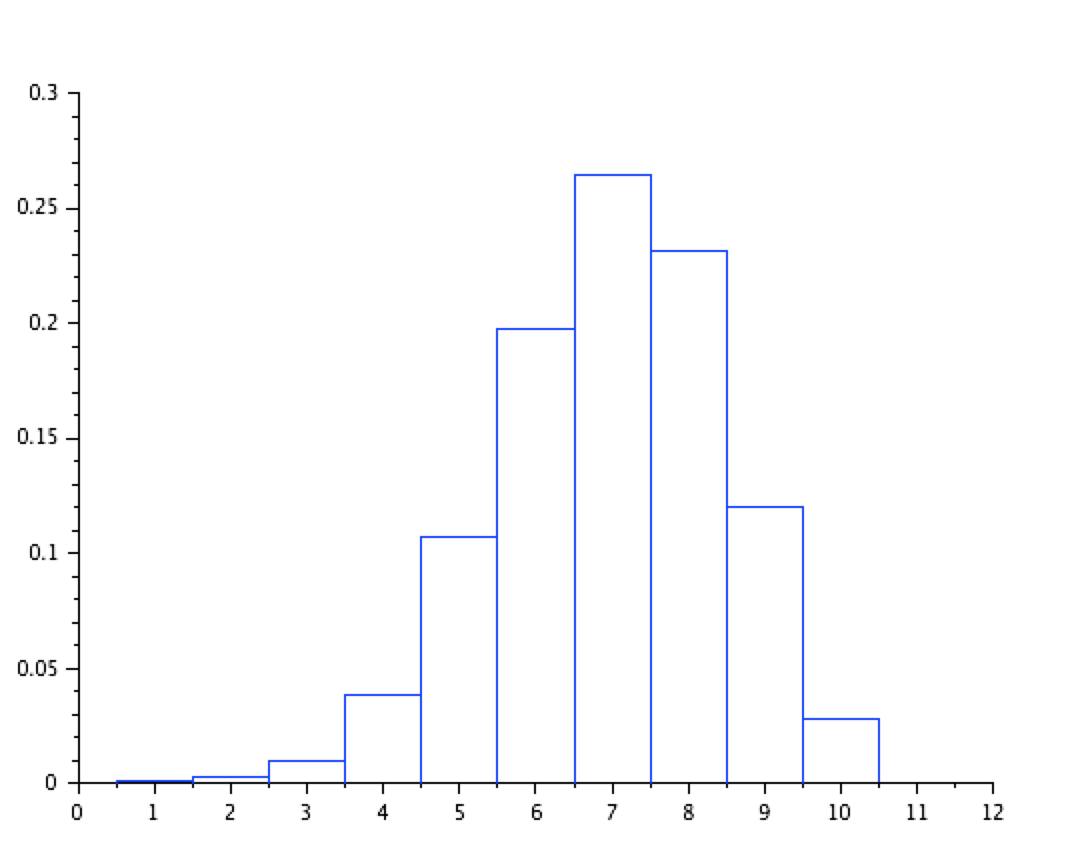
\includegraphics[width=11cm]{S4}
\caption{Histogramme de $X^{*}$ pour $p=0.7$, $M=10$, 5000 lancers}
\label{S4}
\end{figure}

\end{document}
